%%%%%%%%%%%%%%%%%%%%%%%%%%%%%%%%%%%%%%%%%%%%%%%%%%%%%%%%%%%
%% Congratulations, you've made an excellent choice
%% of writing your Tampere University thesis using
%% the LaTeX system. This document attempts to be
%% as complete a template as possible to let you focus
%% on the most important part: the writing itself.
%% Thus the details regarding the visual appearance
%% and even structure have already been worked out
%% for you!
%%
%% I sincerely hope you will find this template useful
%% in completing your thesis project. I've tried to
%% add comments (followed by the % sign) to clarify
%% the structure and purpose of some of the commands.
%% Most of the magic happens in the file tauthesis.cls,
%% which you are more than welcome to take a look at.
%% Just refrain from editing it in the most crucial
%% versions of the thesis!
%%
%% I wish you and your thesis project the best of luck!
%% If this template causes you trouble along the way
%% or if you've any suggestions for improving it,
%% please be in contact through GitHub
%% (<URL HERE>)
%%
%% Yours,
%%
%% Ville Koljonen
%%
%% PS. This template or its associated class file don't
%% come with a warranty. The content is provided as is,
%% without even the implied promise of fitness to the
%% mentioned purpose. You, as the author of the thesis,
%% are responsible for the entire work, including the
%% provided material. No one else is liable to you for
%% any damage inflicted on you or your thesis, were it
%% caused by using this template or not.
%%%%%%%%%%%%%%%%%%%%%%%%%%%%%%%%%%%%%%%%%%%%%%%%%%%%%%%%%%%

%%%%% NOTICE %%%%%
%% Please read through the entire template
%% (files under ./tex) to find all instructions.
%% It is possible that the attached pdf files
%% do not include the latest information.
%%%%%%%%%%%%%%%%%%

%%%%% INSTRUCTIONS FOR COMPILING THE DOCUMENT %%%%%
%% Overleaf: just click Recompile.
%% Terminal:
%%  1. pdflatex main.tex
%%  2. makeindex -s main.ist -t main.glg -o main.gls main.glo
%%  3. biber main
%%  4. pdflatex main.tex
%%  5. pdflatex main.tex
%% Similar sequence of commands is also required
%% in LaTeX specific editors.
%%%%%%%%%%%%%%%%%%%%%%%%%%%%%%%%%%%%%%%%%%%%%%%%%%%

%%% Set PDF version before doing anything else.

%%% set-pdf-version.tex
%
% This file is loaded by main.tex before any other operations, so that PDF
% version is set correctly for accessibility features.
%

\RequirePackage{ifluatex}

\def\mypdfminorversion{6}

\ifluatex

    \directlua {
        if pdf.getminorversion() \string~= \mypdfminorversion then
            if (status.pdf_gone and status.pdf_gone > 0)
            or (status.pdf_ptr and status.pdf_ptr > 0)
            then
                tex.error("PDF version cannot be changed anymore.")
            else
                pdf.setminorversion(\mypdfminorversion)
            end
        end
    }

\else

    \pdfminorversion=\mypdfminorversion

\fi


%%%%% METADATA %%%%%
%
% Always keep the following metadata up to date! This is important for your
% PDF file to comply to accessibility standards. (And yes, this information
% must remain here, before \documentclass[...]{...}.)

\def\myfititle{Dieselmoottorin hiukkassuodattimen tilan estimointi}
\def\myentitle{State Estimation of a Diesel Particulate Filter}
\def\myauthor{Tuomas Haataja}
\def\myfisubtitle{}
\def\myensubtitle{}
\def\myfithesistype{Diplomityö}
\def\myenthesistype{Masters of Science Thesis}
\def\myexaminers{Veli-Pekka Pyrhönen \\ Prof. Matti Vilkko}
\def\myfifacultyname{Tekniikan ja luonnontieteiden tiedekunta}
\def\myenfacultyname{Faculty of Engineering and Natural Sciences}
\def\myfiprogrammename{Automaatiotekniikka}
\def\myenprogrammename{Automation Engineering}
\def\myfikeywords{Hiukkassuodatin, DPF, noki}
\def\myenkeywords{Diesel Particulate Filter, DPF, soot}
\def\mylanguagecode{en-GB}
\def\mysubject{A short description of the thesis subject.}
\def\myyear{2025}
\def\mymonth{08}
\def\myday{31}

% Define your citation options here. Valid values for style and sorting options
% can be found in the BibLaTeX manual: https://ctan.org/pkg/biblatex.

\def\mycitationstyle{numeric}
%\def\mycitationsorting{nyt}
\def\mycitationsorting{none}

%%%%% PREAMBLE %%%%%

%%%%% Document class declaration.
%
% The possible optional arguments are
%
%   finnish - thesis in Finnish (default)
%   english - thesis in English
%   draft - for faster non-final works, also skips images
%           (recommended, remove in final version)
%   programs - if you wish to display code snippets
% Example: \documentclass[english, authoryear]{tauthesis}
%          thesis in English with author-year citations

\documentclass[finnish]{tauthesis}

%%% preamble.tex
%
% This file is for including LaTeX libraries or packages and defining your own
% commands.
%
% NOTE: The glossaries package loaded by tauthesis.cls throws a warning: No
% language module detected for 'finnish'. You can safely ignore this. All
% other warnings should be taken care of, before your thesis is submitted!

%%%%% Your packages.
%
% Before adding packages, see if they can be found in tauthesis.cls already.
% If you're not sure that you need a certain package, don't include it in the
% document! This can dramatically reduce compilation time.

% Graphs
% \usepackage{pgfplots}
% \pgfplotsset{compat=1.15}

% Subfigures and wrapping text
% \usepackage{subcaption}

%% Theorem environments and their numbering.
%
% Define both English and Finnish theorem types. These all follow the same
% counter. See the documentation of amsthm to see how these can be changed to
% suit your needs, if necessary.
%

\usepackage{amsthm}

\theoremstyle{definition}

\newtheorem{definition}{Definition}[chapter]
\newtheorem{theorem}[definition]{Theorem}
\newtheorem{lemma}[definition]{Lemma}
\newtheorem{corollary}[definition]{Corollary}
\newtheorem{example}[definition]{Example}

\newtheorem{maaritelma}[definition]{Määritelmä}
\newtheorem{lause}[definition]{Lause}
\newtheorem{apulause}[definition]{Apulause}
\newtheorem{seurauslause}[definition]{Seurauslause}
\newtheorem{esimerkki}[definition]{Esimerkki}

% Mathematics packages
\usepackage{mathtools, amssymb}
%\usepackage{bm}

% Chemistry packages
% \usepackage{chemfig}
% \usepackage[version=4]{mhchem}

% Text hyperlinking
% \usepackage{hyperref}
% \hypersetup{hidelinks}

% (SI) unit handling
\usepackage{siunitx}

\sisetup{
    detect-all,
    math-sf=\mathrm,
    exponent-product=\cdot,
    output-decimal-marker={,} % for theses in FINNISH!
}

%% For code listings.

\usepackage{listings}

% This global code listing configuration is required for automatically
% replacing special characters with corresponding LaTeX commands, in code files
% included with \lstinputlisting. Without it, letters like 'ä' in code file
% comments will result in a LaTeX errors.
%
% Source: https://tex.stackexchange.com/a/574950.

\lstset{
    inputencoding = utf8,  % Input encoding
    extendedchars = true,  % Extended ASCII
    literate      =        % Support additional characters
        {á}{{\'a}}1  {é}{{\'e}}1  {í}{{\'i}}1 {ó}{{\'o}}1  {ú}{{\'u}}1
        {Á}{{\'A}}1  {É}{{\'E}}1  {Í}{{\'I}}1 {Ó}{{\'O}}1  {Ú}{{\'U}}1
        {à}{{\`a}}1  {è}{{\`e}}1  {ì}{{\`i}}1 {ò}{{\`o}}1  {ù}{{\`u}}1
        {À}{{\`A}}1  {È}{{\`E}}1  {Ì}{{\`I}}1 {Ò}{{\`O}}1  {Ù}{{\`U}}1
        {ä}{{\"a}}1  {ë}{{\"e}}1  {ï}{{\"i}}1 {ö}{{\"o}}1  {ü}{{\"u}}1
        {Ä}{{\"A}}1  {Ë}{{\"E}}1  {Ï}{{\"I}}1 {Ö}{{\"O}}1  {Ü}{{\"U}}1
        {â}{{\^a}}1  {ê}{{\^e}}1  {î}{{\^i}}1 {ô}{{\^o}}1  {û}{{\^u}}1
        {Â}{{\^A}}1  {Ê}{{\^E}}1  {Î}{{\^I}}1 {Ô}{{\^O}}1  {Û}{{\^U}}1
        {œ}{{\oe}}1  {Œ}{{\OE}}1  {æ}{{\ae}}1 {Æ}{{\AE}}1  {ß}{{\ss}}1
        {ẞ}{{\SS}}1  {ç}{{\c{c}}}1 {Ç}{{\c{C}}}1 {ø}{{\o}}1  {Ø}{{\O}}1
        {å}{{\aa}}1  {Å}{{\AA}}1  {ã}{{\~a}}1  {õ}{{\~o}}1 {Ã}{{\~A}}1
        {Õ}{{\~O}}1  {ñ}{{\~n}}1  {Ñ}{{\~N}}1  {¿}{{?`}}1  {¡}{{!`}}1
        {°}{{\textdegree}}1 {º}{{\textordmasculine}}1 {ª}{{\textordfeminine}}1
        {£}{{\pounds}}1  {©}{{\copyright}}1  {®}{{\textregistered}}1
        {«}{{\guillemotleft}}1  {»}{{\guillemotright}}1  {Ð}{{\DH}}1  {ð}{{\dh}}1
        {Ý}{{\'Y}}1    {ý}{{\'y}}1    {Þ}{{\TH}}1    {þ}{{\th}}1    {Ă}{{\u{A}}}1
        {ă}{{\u{a}}}1  {Ą}{{\k{A}}}1  {ą}{{\k{a}}}1  {Ć}{{\'C}}1    {ć}{{\'c}}1
        {Č}{{\v{C}}}1  {č}{{\v{c}}}1  {Ď}{{\v{D}}}1  {ď}{{\v{d}}}1  {Đ}{{\DJ}}1
        {đ}{{\dj}}1    {Ė}{{\.{E}}}1  {ė}{{\.{e}}}1  {Ę}{{\k{E}}}1  {ę}{{\k{e}}}1
        {Ě}{{\v{E}}}1  {ě}{{\v{e}}}1  {Ğ}{{\u{G}}}1  {ğ}{{\u{g}}}1  {Ĩ}{{\~I}}1
        {ĩ}{{\~\i}}1   {Į}{{\k{I}}}1  {į}{{\k{i}}}1  {İ}{{\.{I}}}1  {ı}{{\i}}1
        {Ĺ}{{\'L}}1    {ĺ}{{\'l}}1    {Ľ}{{\v{L}}}1  {ľ}{{\v{l}}}1  {Ł}{{\L{}}}1
        {ł}{{\l{}}}1   {Ń}{{\'N}}1    {ń}{{\'n}}1    {Ň}{{\v{N}}}1  {ň}{{\v{n}}}1
        {Ő}{{\H{O}}}1  {ő}{{\H{o}}}1  {Ŕ}{{\'{R}}}1  {ŕ}{{\'{r}}}1  {Ř}{{\v{R}}}1
        {ř}{{\v{r}}}1  {Ś}{{\'S}}1    {ś}{{\'s}}1    {Ş}{{\c{S}}}1  {ş}{{\c{s}}}1
        {Š}{{\v{S}}}1  {š}{{\v{s}}}1  {Ť}{{\v{T}}}1  {ť}{{\v{t}}}1  {Ũ}{{\~U}}1
        {ũ}{{\~u}}1    {Ū}{{\={U}}}1  {ū}{{\={u}}}1  {Ů}{{\r{U}}}1  {ů}{{\r{u}}}1
        {Ű}{{\H{U}}}1  {ű}{{\H{u}}}1  {Ų}{{\k{U}}}1  {ų}{{\k{u}}}1  {Ź}{{\'Z}}1
        {ź}{{\'z}}1    {Ż}{{\.Z}}1    {ż}{{\.z}}1    {Ž}{{\v{Z}}}1
}

%%%%% Your commands.
\hypersetup{hidelinks} % Remove boxes around links
\usepackage{float}
\usepackage{tikz}
\usetikzlibrary{arrows.meta}
\usetikzlibrary{decorations.pathmorphing,calc,shapes,arrows,snakes,shapes.geometric,patterns,fadings}
\usepackage[version=4]{mhchem}

% Print verbatim LaTeX commands
\newcommand{\verbcommand}[1]{\texttt{\textbackslash #1}}

% Command for formatting code.

\newcommand\code[1]{\texttt{#1}}

% A delimiter command for the norm of a vector with mathtools.

\DeclarePairedDelimiter\norm{\lVert}{\rVert}


% Basic theorems in Finnish and in English.
% Remove [chapter] if you wish a simply
% running enumeration.
% \newtheorem{lause}{Lause}[chapter]
% \newtheorem{theorem}[lause]{Theorem}

% \newtheorem{apulause}[lause]{Apulause}
% \newtheorem{lemma}[lause]{Lemma}

% Use these versions for individually
% enumerated lemmas
% \newtheorem{apulause}{Apulause}[chapter]
% \newtheorem{lemma}{Lemma}[chapter]

% Definition style
% \theoremstyle{definition}
% \newtheorem{maaritelma}{Määritelmä}[chapter]
% \newtheorem{definition}[maaritelma]{Definition}
% examples in this style

%%%%% Glossary information.

% Use the following lines ONLY if you need more
% than one glossary. The first argument specifies
% a type label for the glossary and the second
% the displayed name.
% \newglossary*{symbs}{Symbols}
% \newglossary{label}{Displayed name}
% ...

\makeglossaries

% Use this line if using the default glossary.
% Otherwise comment out.

\loadglsentries[main]{tex/sanasto.tex}

% Use this line if using more than one glossary.
% Otherwise comment out.
% \loadglsentries[symbs]{tex/sanasto2.tex}

%%%%% Citation information.

% Commonly used bibliography modifications.
% Feel free to play around with them.

%\ExecuteBibliographyOptions{%
%sorting=none,
%maxbibnames=99,
%maxcitenames=2,
%giveninits=true,
%uniquename=init,
%sortcites,
%sortlocale=fin}

%\DeclareNameAlias{sortname}{last-first}
%\DeclareNameAlias{author}{last-first}

%\DeclareFieldFormat[%
%    article,inbook,incollection,inproceedings,
%    patent,thesis,unpublished]{citetitle}{#1\isdot}
%\DeclareFieldFormat[%
%    article,inbook,incollection,inproceedings,
%    patent,thesis,unpublished]{title}{#1\isdot}
%\DeclareFieldFormat{pagetotal}{#1 \bibstring{page}}

%\AtBeginBibliography{\renewcommand*{\makelabel}[1]{#1\hss}}

%\DefineBibliographyExtras{english}{\let\finalandcomma=\empty}

\addbibresource{tex/references.bib}
 % You can add packages and define new commands in this file.
\newcommand{\doo}{\partial}

%\makeglossaries
\begin{document}

%%%%% FRONT MATTER %%%%%

\frontmatter

%%%%% Thesis information and title page.

% Enable the use of @ character in command names.

\makeatletter

% The titles of the work. If there is no subtitle, leave the \myfisubtitle or
% \myensubtitle command arguments empty. Pass the title in the primary
% language as the first argument and its translation to the secondary language
% as the second.

\if@langenglish

    \title{\myentitle}{\myfititle}

\else

    \title{\myfititle}{\myentitle}

\fi

\if@langenglish

    \subtitle{\myensubtitle}{\myfisubtitle}

\else

    \subtitle{\myfisubtitle}{\myensubtitle}

\fi

% The author name.

\author{\myauthor}

% The examiner information. If your work has multiple examiners, replace with
%
%   \examiner[<label>]{<name> \\ <name>}
%
% where <label> is an appropriate (plural) label, e.g. Examiners or
% Tarkastajat, and <name>s are replaced by the examiner names, each on their
% separate line.

\examiner{\myexaminers}

% The finishing date of the thesis (YYYY-MM-DD).

\finishdate{\myyear}{\mymonth}{\myday}

% The type of the thesis (e.g. Kandidaatintyö or Master of Science Thesis) in
% the primary and the secondary languages of the thesis.

\if@langenglish

    \thesistype{\myenthesistype}{\myfithesistype}

\else

    \thesistype{\myfithesistype}{\myenthesistype}

\fi

% The faculty and degree programme names in the primary and the secondary
% languages of the thesis, respectively.

\if@langenglish

    \facultyname{\myenfacultyname}{\myfifacultyname}

\else

    \facultyname{\myfifacultyname}{\myenfacultyname}

\fi

\if@langenglish

    \programmename{\myenprogrammename}{\myfiprogrammename}

\else

    \programmename{\myfiprogrammename}{\myenprogrammename}

\fi

% The keywords of the thesis in the primary and the secondary languages of the
% thesis.

\if@langenglish

    \keywords{\myenkeywords}{\myfikeywords}

\else

    \keywords{\myfikeywords}{\myenkeywords}
\fi

% Make @ a regular letter again.

\makeatother

% Actually generate the title page based on the above commands.

\maketitle


%%%%% Abstracts and preface.
%
% Write the abstract(s) and the preface into a separate file for the sake of
% clarity. Pass the appropriate file name as the first argument to these
% commands. Put the \abstract in the primary language first and the
% \otherabstract in the secondary language second. Those who do not speak
% Finnish only need the first abstract. The second argument of the \preface
% command takes the place where the thesis was signed in.
%
% Edit the files tex/{use-of-ai,tekoalyn-kaytto}.tex to match your use of AI in
% generating this thesis.
%

\abstract{tex/tiivistelma.tex}

\otherabstract{tex/abstract.tex}

\aidisclaimerinclusioncmd

\preface{tex/alkusanat.tex}{Tampereella}

%%%%% Table of contents.

\tableofcontents

%%%%% Lists of figures, tables, listings and terms.
%
% Print the lists of figures and/or tables. Uncomment either of these commands
% as required. Both are optional, but if there are many important
% figures/tables, listing them may be a good idea.

% \listoffigures
% \listoftables
% \lstlistoflistings

% Misc stuff related to how the glossary is displayed. You can especially
% tweak the lengths to suit you!

\glsaddall
\setglossarystyle{taulong}
\setlength{\glsnamewidth}{0.25\textwidth}
\setlength{\glsdescwidth}{0.75\textwidth}
\renewcommand*{\glsgroupskip}{}

% Print the default glossary of abbreviations, if necessary. Otherwise comment
% out. The appropriate Finnish variant is 'Lyhenteet'

\printglossary[title={Lyhenteet ja merkinnät}]

%\printglossaries
% Print more than one glossary with these lines. Otherwise comment out.

% \printglossary[type=symbs]
% \printglossary[type=label]
% ...

%%%%% MAIN MATTER %%%%%

\mainmatter

% Write each of the chapters of the thesis into a separate file for the sake
% of clarity. They can be \input as shown below. Give both the chapters and
% their files as descriptive names as possible.

\chapter{Johdanto}%
\label{ch:johdanto}
Dieselmoottori on muun muassa toimintavarmuutensa ja energiatehokkuutensa vuoksi yksi nykypäivän merkittävimmistä voimanlähteistä muun muassa työkoneissa \cite[s. 121, 137-138]{Koten_2024}.
Pelkästään Yhdysvalloissa noin 75\% maatalouden työkoneista käyttää dieselmoottoria voimanlähteenään \cite[s. 122]{Koten_2024}.  
Dieselmoottori kuitenkin tuottaa palamisolosuhteiden vuoksi
huomattavasti päästöjä \cite{FiebigMichael2014Pefd}. Erityisesti typen oksidit (NO\(_x\)) ja hiukkaspäästöt ovat ongelma niin terveydelle kuin ympäristöllekin \cite[s. 138]{Koten_2024}\cite{YaoDongwei2023Rodm}, joten  lainsäädäntö asettaa yhä tiukentuvat rajat dieselmoottorien päästöille. Tämän vuoksi moderneissa työkoneissa on käytettävä pakokaasun jälkikäsittelyjärjestelmiä, jotka pyrkivät vähentämään dieselmoottorin tuottamien haitallisten päästöjen pääsyä ilmakehään. Koska lainsäädännön rajat tiukentuvat, täytyy jälkikäsittelyjärjestelmiä kehittää ja parantaa jatkuvasti.

Hiukkaspäästöjä voidaan pienentää merkittävästi hiukkassuodattimella (DPF, \emph{eng. Diesel Particulate Filter}).
Tyypillisin DPF-järjestelmän rakenne on hunajakennomainen sylinteri, jossa on vuoronperään eri päistä suljettuja putkia \cite{SHIYunxi2020Eota}. Putkien välillä on huokoiset seinämät, joiden läpi pakokaasu pääsee virtaamaan. {\color{red} TODO}

DPF suodattaa läpivirtaavasta pakokaasusta hiilestä ja hiilivedyistä koostuvan noen sekä palamattomasta materiaalista koostuvan tuhkan huokoisiin seinämiin ja niiden pinnalle. {\color{red} TODO}

DPF-järjestelmään kertynyt noki ja tuhka tulee aika ajoin poistaa. Tuhka poistetaan manuaalisella puhdistuksella, mutta nokea voidaan hapettaa hiilidioksidiksi hapen ja typen oksidien avulla. Tätä kutsutaan regeneroinniksi, joka jaetaan karkeasti passiiviseen ja aktiiviseen regenerointiin.
Aktiivisen regeneroinnin ajoitus on syytä toteuttaa oikeaan aikaan, sillä liian aikainen regenerointi kuluttaa ylimäärin polttoainetta, kun taas liian myöhäinen nostaa vastapainetta, mikä voi olla jopa vaarallista \cite{YaoDongwei2023Rodm}. 
Näin ollen DPF-järjestelmän tila -- erityisesti noen  määrä -- on syytä tuntea mahdollisimman tarkasti. 

Nokilatausta arvioidaan painehäviömittauksilla ja hiukkaslukumäärää kuvaavaan matemaattisfysikaaliseen malliin perustuvalla ennusteella \cite{YaoDongwei2023Rodm}. Painehäviömittaus on kuitenkin herkkä häiriöille ja vikaantumiselle, eikä se kykene erottelemaan nokea ja tuhkaa toisistaan.
Toisaalta mallin ennusteen virhe kumuloituu ajan myötä \cite{YaoDongwei2023Rodm}.
Tämän työn tarkoituksena on toteuttaa näitä arvioita yhdistelemällä hyvä nokilatausestimaatti. 

Hiukkassuodattimeen kertyneen tuhkan määrää arvioidaan mallipojaisesti \cite{??}. 
Kertynyt tuhka aiheuttaa painemittaukseen kasvavan trendin. Työssä on tarkoitus toteuttaa estimointimenetelmä tuhkalataukselle painemittaukseen perustuen.{\color{red} TODO}

Estimointiin käytetään Bayesilaisia suotimia, erityisesti Kalman-suodinta. Hiukkassuodatinta mallintavien yhtälöiden epälineaarisuuden vuoksi työssä tarkastellaan Kalman-suo-timen epälineaarisia versioita, kuten laajennettua Kalman-suodinta (EKF, \emph{Extended Kalman Filter}).{\color{red} TODO}

Työssä ei suoriteta uusia mittauksia, vaan käytetään usean kenttäkäyttöisen koneen moottorinohjausyksikön (ECU, \emph{eng. Engine Control Unit}) keräämää dataa. {\color{red} TODO}

Työn tavoitteena on selvittää, kuinka paljon hapettavan katalysaattorin \(\ce{NO}_x\)-mallin virhe aiheuttaa epävarmuutta DPF-tilan estimaattiin. Epävarmuutta mallinnetaan tilan todennäköisyysjakauman varianssina. Toisaalta kiinnostavaa on myös selvittää, kuinka paljon hiukkassuodattimen käyttöolosuhteet, kuten lämpötila vaikuttavat DPF-tilan varianssiin. 

Luvussa 2 esitellään hiukkassuodatin yksityiskohtaisesti osana jälkikäsittelyjärjestelmää.
Luvussa 3 esitellään yleisesti systeemin tilan estimointimenetelmiä, erityisesti Kalman-suodin ja sen laajennuksia.
Luvussa 4 toteutetaan luvun 3 mukainen estimointimenetelmä hiukkassuodattimen tilan estimoinniksi. Luvussa 5 tarkastellaan saatuja tuloksia.

\chapter{Hiukkassuodatin}%
\label{ch:dpf}



Dieselmoottorin hiukkassuodatin, eli DPF (\emph{eng. Diesel Particulate Filter}) on tehokkain järjestelmä pakokaasun noki- ja tuhkapartikkeleiden suodatukseen. 
Hyvä DPF suodattaa läpivirtaavasta pakokaasusta jopa 99\% hiukkaslukumäärästä ja 95\% -massasta \cite{Yan_state_of_the_art}. Hiukkassuodatin on osa useammasta komponentista koostuvaa jälkikäsittelyjärjestelmää, jota on havainnollistettu Kuvassa \ref{fig:EAT_full}. %

\begin{figure}[H]
    \centering
    \pdftooltip{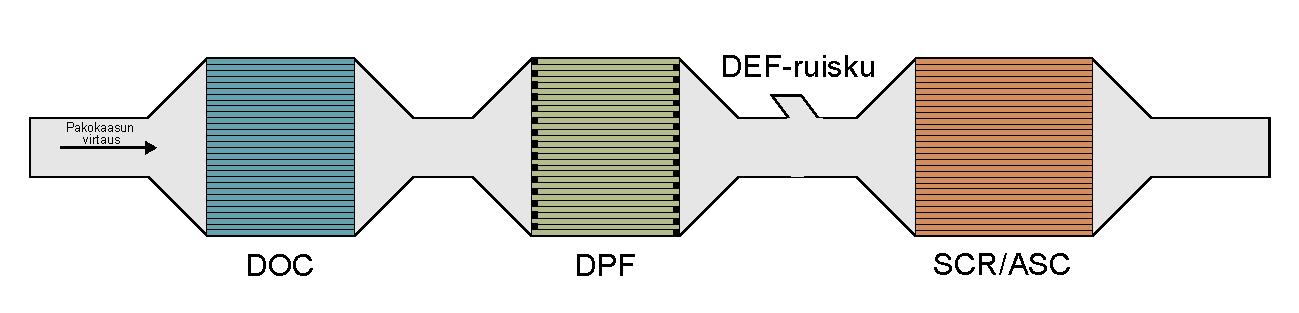
\includegraphics[width=\textwidth]{figures/EAT2.pdf}}
                {Kuvituskuva jälkikäsittelyjärjestelmästä. Kuvaan merkitty hapetuskatalysaattori, hiukkassuodatin ja selektiivinen katalyyttinen pelkistin.}
    \caption{Modernin jälkikäsittelyjärjestelmän osat.}
    \label{fig:EAT_full}
\end{figure}

Moderni jälkikäsittelyjärjestelmä koostuu yleensä hapettavasta katalysaattorista (DOC, \emph{eng. Diesel Oxidation Catalyst}), hiukkassuodattimesta (DPF), sekä selektiivisestä katalyyttisestä pelkistimestä (SCR, \emph{eng. Selective Catalytic Reduction}). Hapettavan katalysaattorin tehtävä on nimensä mukaan hapettaa moottorin päästöjä, kuten hiilivetyjä, häkää, ja tämän työn kannalta olennaista typpimonoksidia \cite{dieselnet_doc}. SCR puolestaan pelkistää ympäristölle ja terveydelle haitalliset typen oksidit typpikaasuksi ja vedeksi \cite{dieselnet_scr}.



\section{Järjestelmän fyysinen rakenne}

Tyypillisin DPF-tyyppi on ns. seimämävirtaus-DPF (\emph{eng. wall-flow DPF}), jossa pakokaasu virtaa hunajakennomaisessa suodattimessa puoliavoimissa putkissa. Pakokaasu virtaa putkien välillä huokoisten seinämien läpi. Pakokaasun hiukkaset jäävät kiinni seinämien sisään ja pinnalle. Virtausta on havainnollistettu Kuvassa \ref{fig:wall-flow-dpf}  


\begin{figure}[H]
    \centering 
    \pdftooltip{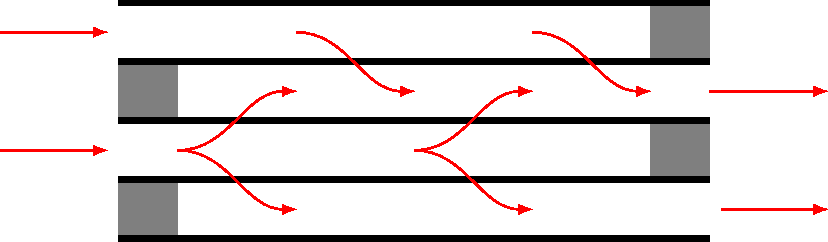
\includegraphics[width=\textwidth]{figures/wall_flow_DPF_figure.pdf}}
               {Kuvituskuva hiukkassuodattimen toiminnasta. Nuolilla kuvattu pakokaasu virtaa avoimiin putkiin ja kulkee seinämien läpi.}
    \caption{Pakokaasu virtaa suodattimessa huokoisten seinämien läpi. Yli 90\% pakokaasun hiukkasmassasta jää huokoisten seinämien sisään ja pinnalle. Mukailtu lähteestä \cite{dieselnet_dpf}.}
    \label{fig:wall-flow-dpf}
\end{figure}

Tässä työssä noen kerääntymistä seinämien sisään ja pinnalle ei erotella, vaan oletetaan nokimäärän kerääntyvän homogeeniseksi kerrokseksi.


\section{Regenerointi}
Noen poistoa suodattimesta hapettamalla kutsutaan regeneroinniksi. Regenerointi jaetaan karkeasti kahteen tapaan: aktiiviseen ja passiiviseen regenerointiin. 
Aktiivinen regenerointi tarkoittaa käytännössä noen polttamista ja se
vaatii korkean, yli 600:n \degree C lämpötilan. Tarvittava energia saadaan ajoneuvon polttoainetta käyttämällä \cite{dieselnet_dpf}. Passiiviseen regenerointiin riittää huomattavasti matalammat lämpötilat ja se perustuu noen hapetusreaktioihin typpidioksidin (NO\(_2\)) kanssa. Tarvittava typpidioksidi saadaan hapettamalla moottorin raakapäästöinä muodostuvaa typpimonoksidia (NO) hapettavassa katalysaattorissa (DOC, \emph{Diesel Oxidation Catalyst}).


Regenerointia kuvaavat reaktioyhtälöt ovat  
\begin{align}
    \ce{C + 1/2 O2 &-> CO }\label{req:regen_c2co}\\
    \ce{C + O2 &-> CO2}\label{req:regen_c2co2}\\
    \ce{C + NO2 &-> CO +  NO}  \\
    \ce{C + 2 NO2 &-> CO2 + 2 NO}  \\
    \ce{C + NO2 + 1/2 O2 &-> CO2 + NO} \text{ ja }\\
    \ce{C + NO2 + 1/2 O2 &-> CO + NO2},
\end{align}
ja niiden reaktionopeudet voidaan määrittää Arrheniuksen yhtälöinä \cite{LiuGuanlin2021Roio}.

\section{Hiukkassuodattimen matemaattinen esitys}

% \begin{figure}[H]
%     \centering 
%     \begin{tikzpicture}
    % Draw the first rectangle
    \node[draw, rectangle, minimum width=1.5cm, minimum height=3cm] (rect1) at (0, 0) {Rectangle 1};

    % Draw the second rectangle
    \node[draw, rectangle, minimum width=1.5cm, minimum height=3cm] (rect2) at (4, 0) {Rectangle 2};

    % Draw arrows between rectangles
    \draw[-{Latex}, thick] ([yshift=-0.5cm]rect1.north east) -- ([yshift=-0.5cm]rect2.north west);
    \draw[-{Latex}, thick] ([yshift=0.5cm]rect1.south east) -- ([yshift=0.5cm]rect2.south west);

    % Draw inputs to rect1
    \draw[-{Latex}, thick] (-3, 1) -- ([yshift=1cm]rect1.west) node[above left] {Nokilataus (g/l)};
    \draw[-{Latex}, thick] (-3, -1) -- ([yshift=-1cm]rect1.west) node[below left] {Tuhkalataus (g/l)};

    % Draw output from rect2
    \draw[-{Latex}, thick] (rect2.east) -- (7, 0) node[above right] {Paine (hPa)};

\end{tikzpicture}
%     \caption{}
%     \label{fig:blocks1}
% \end{figure}

Suodattimen painehäviötä mallinnetaan useimmiten Darcyn lain, tai Forcheimer-Darcyn yhtälöiden avulla \cite{dieselnet_wall_flow_monolith}.

\begin{align}
    Q = \frac{\dot{m}}{\rho(T)}.
\end{align}

Suodattimen sisäänmenossa painehäviö
\begin{align}
    \Delta P_{inlet} = \frac{1}{6} \cdot
    Q \cdot \mu(T) 
    \cdot F \cdot \frac{L^2}{V} \cdot \frac{(\alpha_{in}-\alpha_{out}+2 d_{wall})^2}{(\alpha_{in}-2d_{soot}-2d_{ash})^4}.
    \label{eq:PDinletchannel}
\end{align}

Suodattimen ulostulossa painehäviö
\begin{align}
    \Delta P_{outlet} = \frac{1}{6} \cdot
    Q \cdot \mu(T) 
    \cdot F \cdot \frac{L^2}{V} \cdot \frac{(\alpha_{in}-\alpha_{out}+2 d_{wall})^2}{\alpha_{out}^4}.
    \label{eq:PDoutletopen}
\end{align}

Suodattimen sisällä painehäviö 
\begin{align}
    \Delta P_{wall} = \frac{1}{4} \cdot
    Q \cdot \mu(T) 
    \cdot \frac{d_{wall}}
    {n_{open}\cdot L \cdot \kappa_{wall} \cdot \alpha_{out}}.
    \label{eq:PDfilterwall}
\end{align}

Nokikerroksen aiheuttama painehäviö
\begin{align}
    \Delta P_{soot} =  \frac{1}{8} \cdot
    Q \cdot \mu(T) \cdot 
    \frac{\ln{\frac{\alpha_{out}-2d_{ash}}{\alpha_{out}-2d_{soot}-2d_{ash}}}}
    {n_{open}\cdot L \cdot \kappa_{soot}}.
    \label{eq:PDsootlayer}
\end{align}

Tuhkakerroksen aiheuttama painehäviö
\begin{align}
    \Delta P_{ash} = \frac{1}{8} \cdot
    Q \cdot \mu(T) \cdot 
    \frac{\ln{\frac{\alpha_{out}}{\alpha_{out}-2d_{ash}}}}
    {n_{open}\cdot L \cdot \kappa_{ash}}.
    \label{eq:PDashlayer}
\end{align}

Kokonaispainehäviö
\begin{align}
    \Delta P_{tot}  = \Delta P_{inlet} +  \Delta P_{outlet} + \Delta P_{wall} + \Delta P_{soot} +  \Delta P_{ash}.
\end{align}

\chapter{Systeemin tilan estimointi }%Bayesilaisilla suotimilla}%
\label{ch:estimointi}
Optimaaliset suotimet ovat  matemaattisia menetelmiä, joilla estimoidaan systeemien tiloja kohinaisiin mittauksiin perustuen \cite{sarkka_bayesian}. Tässä työssä tarkastellaan Bayesilaisia suotimia, jotka ratkaisevat optimointiongelman Bayesilaisittain. 

\section{Teoreettista taustaa}
{\color{red} (nimi vaihtuu), Lyapunov ja Riccati yms.}

\section{Kalman-suodin}

Kalman-suodin on algoritmi, jolla voidaan estimoida lineaarisen ja kohinaisen systeemin tilaa. Systeemin kohinan tulee olla valkoista kohinaa \cite[s. 56]{sarkka_bayesian}. Algoritmi on kaksivaiheinen ja se koostuu ennuste- ja päivitysvaiheista. 
Ennustevaihe tehdään lähtökohtaisesti jokaisella aika-askeleella. Päivitysvaihe sen sijaan voidaan laskennan tai saavuttamattoman mittauksen vuoksi toteuttaa harvemminkin. 

Tarkastellaan lineaarista systeemiä
\begin{align}
    \begin{split}
        x_k &= A_{k-1}x_{k-1} + w_{k-1} \\
        y_k &= H_k x_k + v_k,
    \end{split}
\end{align}
jossa \(x_k \in \R^n \) on systeemin tila hetkellä \(k\), \(A_{k-1}\in \R^{n\times n}\) on tilamatriisi, \(y_k\in \R^m\) on mittaus, \(H_k \in \R^{m \times n}\) on mittausmatriisi. Muuttujat \(w_{k-1} \sim \mathcal{N}(0, Q_{k-1})\) ja \(v_k \sim \mathcal{N}(0, R_k)\) ovat normaalijakautuneet (Gaussiset) prosessi- ja mittauskohinat, joissa \(Q_{k-1}\) ja \(R_k\) ovat vastaavat kovarianssimatriisit. Tilan ja mittauksen estimaatteja merkitään \(\hat{x}_k\) ja \(\hat{y}_k\).

Kalman-suodin ratkaisee jokaisella iteraatiolla normaalijakautuneen estimaatin, jossa keskiarvo on \(\hat{x}_k\) ja optimoitu kovarianssi on \(P_k\).  

Ennustevaihe:
\begin{align}
    \hat{x}_{k | k-1}  &= A_{k-1} \hat{x}_{k-1}\\
    P_{k | k-1} &= A_{k-1} P_{k-1} A_{k-1}^T + Q_{k-1}.
\end{align}

Päivitysvaihetta varten tarvitaan mittausennuste
\begin{align}
    \hat{y}_k = H_k \hat{x}_{k | k-1} 
\end{align}
ja Kalman-vahvistus 
\begin{align}
    K_k = P_{k | k-1} H_k^T \left(H_k P_{k | k-1} H_k^T + R_k \right)^{-1}.
\end{align}
Kalman-vahvistuksen yhtälö minimoi todellisen ja estimoidun tilan keskiarvon neliöllisen virheen \cite{sparse_kalman_gain}, ja se määrittää kuinka paljon uuteen mittaukseen uskotaan vanhaan estimaattiin verrattuna \cite{becker2023kalman}.

Päivitysvaihe:
\begin{align}
    \hat{x}_{k | k} &= \hat{x}_{k | k-1} + K_k (y_k - \hat{y}_k)\\
    P_{k|k}         &= (I - K_k H_k)P_{k|k-1},
\end{align}
jossa \(I \in \R^{n\times n}\) on identiteettimatriisi.

\section{EKF}
Toisin kuin tavallinen Kalman-suodin, laajennettu Kalman-suodin, eli EKF \emph{(eng. Extended Kalman Filter)} kykenee ratkaisemaan epälineaaristen funktioiden optimointiongelman lähes optimaalisesti. Menetelmä perustuu funktioiden linearisointiin, joten ratkaisu ei välttämättä ole täysin optimaalinen, mutta usein riittävän optimaalinen. Menetelmä kuitenkin vaatii funktioiden derivoituvuutta, sillä algoritmissa ratkaistaan sekö tilanfunktion että mittausfunktion Jacobin matriisit joka iteraatiolla. Tarkastellaan diskreettiä systeemiä, jonka tilanyhtälö on
\begin{align}
    x_k = f(x_{k-1}, u_{k-1}) + w_{k-1},
\end{align}
ja mittausyhtälö on
\begin{align}
    z_k = h(x_{k}, u_{k}) + v_k.
\end{align}
Funktiot \(f\) ja \(h\) ovat yleisesti epälineaarisia ja derivoituvia. Prosessi- ja mittaushäiriöt \(w\) ja \(v\) ovat nollakeskiarvoisia ja normaalijakautuneita, ja niiden kovarianssimatriiseita merkitään \(Q\) ja \(R\).

Kuten tavallisellakin Kalman-suotimella, EKF-algoritmi voidaan jakaa ennuste- ja päivitysvaiheisiin. 
Ennustevaiheessa ratkaistaan uusi estimaatti sekä sen kovarianssimatriisi. Ennustevaihe on muotoa
\begin{align}
    \hat{x}_{k|k-1} &= f(\hat{x}_{k-1|k-1}, u_{k-1}) \\
    P_{k|k-1} &= F_k P_{k-1|k-1} F_k^T + Q_{k-1},
\end{align}
jossa \(F\) on funktion \(f\) Jacobin matriisi. 
Päivitysvaiheessa tilan päivitystä varten ratkaistaan Kalman-vahvistus
\begin{align}
    S_k &= H_k P_{k|k-1} H_k^T + R_k \\
    K_k &= P_{k|k-1} H_k^T S_k^{-1},
\end{align}
jossa \(H\) on funktion \(h\) Jacobin matriisi. 
Kalman-vahvistuksella ja mittauksen ja mallin välisellä virheellä  \(e_{z, k} = z_k - h(\hat{x}_{k|k-1}) \) 
voidaan päivittää estimaatti ja sen kovarianssi
\begin{align}
    \hat{x}_{k|k} &= \hat{x}_{k|k-1} + K_k e_{z, k}, \\
    P_{k|k} &= (I-K_k H_k) P_{k|k-1}.
\end{align}
Kalman-vahvistuksen epäoptimaalisuus johtuu linearisointien epätarkkuudesta. Täten EKF ei ole luotettava estimointialgoritmi pitkille aikaikkunoille, hitaille näytteenottotaajuuksille tai huonosti derivoituville funktioille.

\chapter{Hiukkassuodattimen tilan estimointi}%
\label{ch:dpf_estimointi}

Inputit:
\begin{align*}
    m_{soot, in}\\
    m_{ash, in}\\
    c_{NO_x, in}
\end{align*}

Lämpötila tunnetaan tarkasti, joten se voidaan jättää mallin parametriksi. 

Painehäviömallin funktiot ovat derivoituvia kaikkialla. Näin ollen EKF-algoritmin linearisointi voidaan toteuttaa Newtonin menetelmää hyödyntäen. Funktioiden linearisointi on toteutettu liitteessä \ref{ch:linearisointi}

\chapter{Tulokset}%
\label{ch:tulokset}

\chapter{Yhteenveto}%
\label{ch:yhteenveto}





%%%%% Bibliography/references.

% Print the bibliography according to the information in ./tex/references.bib
% and the in-line citations used in the body of the thesis.

% \emergencystretch=2em
\printbibliography[heading=bibintoc]

%%%%% Appendices.

% Use only if it clarifies the structure of the document. Remember to
% introduce each appendix and its content.

\begin{appendices}


\chapter{Painehäviömallin linearisointi}%
\label{ch:dP_linearisointi}

Tässä liitteessä johdetaan painehäviömallin yhtälöiden linearisointi. Yleisesti linearisointi kohdassa \(x_e\) voidaan esittää muodossa
\begin{align}
    %\tilde{f}(x) = f(x_e) +\sum_{k=1}^n \frac{\doo f(x_e)}{\doo x_k} (x_k-x_e),
    \tilde{f}(x) = f(x_e) +J_f (x_e) (x_k-x_e),
\end{align}
jossa \(x, x_e \in \R^k\) ja \(J_f\) on funktion \(f\) Jacobin matriisi. 
Kokonaispainehäviön termeistä vain \(\Delta P_{inlet}\), \(\Delta P_{soot}\) ja \(\Delta P_{ash}\) riippuvat noki- ja tuhkakerroksista \(w_{soot}\) ja \(w_{ash}\). 
Linearisointi toteutetaan muuttujien \(m_{ash}\) ja \( m_{soot}\) suhteen, joten
sovelletaan yleistä ketjusääntöä Jacobin matriiseille
\begin{align}
    J_{f \circ g}(x) = J_f\big(g(x)\big)  J_g(x).
\end{align}
% \(    J_{f \circ g}(x) = J_f\big(g(x)\big)  J_g(x).\)
Olkoon \(m = \left(m_{soot}, m_{ash}\right) \in \R^2\) ja \(w(m) = \big(w_{soot}(m), w_{ash}(m)  \big) \in \R^2\). Laaditaan funktion \(w\) Jacobin matriisi
\begin{align}
    J_w(m)=
    \bm{
        \frac{\doo w_{soot}}{\doo m_{soot}}
        & 
        \frac{\doo w_{soot}}{\doo m_{ash}} 
        \\  
        \frac{\doo w_{ash}}{\doo m_{soot}}
        & 
        \frac{\doo w_{ash}}{\doo m_{ash}} 
    }.
\end{align}
%joka vastaa derivaattaa.
 Funktion \(\Delta P_{tot}\) Jacobin matriisi puolestaan on 
\begin{align}
    J_{\Delta P_{tot}}(w) = \bm{  
        \frac{\doo \Delta P_{tot}}{\doo w_{soot}}
        &   
        \frac{\doo \Delta P_{tot}}{\doo w_{ash}}
    }.
\end{align}
Näin ollen 
\begin{align}\label{eq:jacob_total_general}
    \begin{split}
        J_{\Delta P_{tot}}(m)&=
        J_{\Delta P}\big(w(m)\big)  J_{w}(m)
\\ &=
    \bm{  
        \frac{\doo \Delta P_{tot}}{\doo w_{soot}}
        &   
        \frac{\doo \Delta P_{tot}}{\doo w_{ash}}
        }
    \bm{
        \frac{\doo w_{soot}}{\doo m_{soot}}
        & 
        \frac{\doo w_{soot}}{\doo m_{ash}} 
        \\ 
        \frac{\doo w_{ash}}{\doo m_{soot}}
        & 
        \frac{\doo w_{ash}}{\doo m_{ash}} 
        }
\\ &=
    \bm{
        \frac{\doo \Delta P_{tot}}{\doo w_{ash}}
        \frac{\doo w_{ash}}{\doo m_{soot}}
        +
        \frac{\doo \Delta P_{tot}}{\doo w_{soot}}
        \frac{\doo w_{soot}}{\doo m_{soot}}
        &
        \frac{\doo \Delta P_{tot}}{\doo w_{ash}}
        \frac{\doo w_{ash}}{\doo m_{ash}}
        +
        \frac{\doo \Delta P_{tot}}{\doo w_{soot}}
        \frac{\doo w_{soot}}{\doo m_{ash}}
        } 
\\ &= 
    \bm{
        \frac{\doo \Delta P_{tot}}{\doo m_{soot}}
        & 
        \frac{\doo \Delta P_{tot}}{\doo m_{ash}} 
        }.
    \end{split}
\end{align}
% Linearisointi on muotoa
% \begin{align}
%     \begin{split}
%     \Delta\tilde{ P}_{tot} &= \Delta P_{tot}
%     +
%     \frac{\doo {\Delta P}_{tot}}{\doo m_{ash}} \Delta m_{ash}
%     + 
%     \frac{\doo {\Delta P}_{tot}}{\doo m_{soot}}  \Delta m_{soot},
% \end{split}
% \end{align}
% joten r
Ratkaistaan Jacobin matriisi 
derivoimalla yhtälöt 
\eqref{eq:deltaP_soot} ja \eqref{eq:deltaP_ash}
noki- ja tuhkalatauksen suhteen. 
% Tuhkakerroksen paksuuden linearisointi on 
% \begin{align}
%     \tilde{w}_{soot}( m_{ash},  m_{soot}) = \frac{\doo w_{soot}}{\doo m_{ash}}  \Delta m_{ash}
%                                                     + \frac{\doo w_{soot}}{\doo m_{soot}} \Delta m_{soot},
% \end{align} 
% ja nokikerroksen 
% \begin{align}
%     \tilde{w}_{ash}( m_{ash},  m_{soot}) = \frac{\doo w_{ash}}{\doo m_{ash}}  \Delta m_{ash}
%                                                     + \frac{\doo w_{ash}}{\doo m_{soot}} \Delta m_{soot}.
% \end{align}
% Yhtälö ei riipu noen määrästä, joten
% \begin{align}
%     \tilde{w}_{soot}( m_{ash},  m_{soot}) =  \frac{\Delta m_{soot}}
%     {4L n_{open} \rho_{soot}\sqrt{\alpha_{in}^2 - \frac{m_{soot, 0}}{L n_{open} \rho_{soot}}}}.
% \end{align}

% Nokikerroksen paksuuteen vaikuttaa myös tuhkakerroksen paksuus. Sijoittamalla yhtälö \eqref{eq:deltaP_wsoot} yhtälöön \eqref{eq:deltaP_wash}, saadaan
% \begin{align}
%     w_{ash}(m_{ash}, m_{soot}) =
%     \frac{ \sqrt{\alpha_{in}^2 - \frac{m_{soot}}{L n_{open} \rho_{soot}}}
%             - 
%            \sqrt{\alpha_{in}^2 - \frac{m_{soot}}{L n_{open} \rho_{soot}} - \frac{m_{ash}}{L n_{open} \rho_{ash}}} }
%     {2}.
% \end{align}

% \begin{align}
%     \begin{split}
%     \tilde{w}_{ash}(m_{ash}, m_{soot}) = &
%     \frac{\Delta m_{ash}}{4 L n_{open} \rho_{{ash}} \sqrt{a_{{in}}^2 - \frac{m_{{soot,0}}}{L n_{open} \rho_{{soot}}} - \frac{m_{{ash,0}}}{L n_{open} \rho_{{ash}}}}} + \\
%     & \frac{\Delta m_{soot}}{4 L n_{open} \rho_{{soot}} \sqrt{a_{{in}}^2 - \frac{m_{{soot,0}}}{L n_{open} \rho_{{soot}}} - \frac{m_{{ash,0}}}{L n_{open} \rho_{{ash}}}}} - \\ &
%     \frac{\Delta m_{soot}}{4 L n_{open} \rho_{{soot}} \sqrt{a_{{in}}^2 - \frac{m_{{soot,0}}}{L n_{open} \rho_{{soot,0}}}}}
%     \end{split}
% \end{align}

% Paremmin näin


% \begin{align*}
%     a &:= 4 L n_{open}, \\
%     b &:= \sqrt{\alpha_{in}^2 - \frac{m_{soot}}{L n_{open} \rho_{soot}}}, \\
%     c &:= \sqrt{\alpha_{in}^2 - \frac{m_{soot}}{L n_{open} \rho_{soot}} - \frac{m_{ash}}{L n_{open} \rho_{ash}}}, \\
%     d &:= \alpha_{in} + \alpha_{out} + w_s,\\
%     f &:= \alpha_{out}- 2 w_{soot},\\
%     q &:= \frac{1}{2}Q\mu,\\
%     \alpha_{in}^* &:= \alpha_{in} - 2 w_{soot} - 2 w_{ash} , \\
%     \alpha_{out}^* &:= \alpha_{out} - 2 w_{soot}  - 2 w_{ash}.
% \end{align*}

% Esitellään apumuuttujat
% \begin{center}
% \begin{tabular}{ll}
%     \( a := 4 L n_{open} \) & \( f := \alpha_{out} - 2 w_{soot} \) \\
%     \( b := \sqrt{\alpha_{in}^2 - \frac{m_{soot}}{L n_{open} \rho_{soot}}} \) & \( q := \frac{1}{2} Q \mu \) \\
%     \( c := \sqrt{\alpha_{in}^2 - \frac{m_{soot}}{L n_{open} \rho_{soot}} - \frac{m_{ash}}{L n_{open} \rho_{ash}}} \) & \( \alpha_{in}^* := \alpha_{in} - 2 w_{soot} - 2 w_{ash} \) \\
%     \( d := \alpha_{in} + \alpha_{out} + 2w_s \) & \( \alpha_{out}^* := \alpha_{out} - 2 w_{soot} - 2 w_{ash} \)
% \end{tabular}
% \end{center}


% Tuhkakerroksen derivaatat ovat
% \begin{align}
%     \frac{\doo w_{soot}}{\doo m_{ash}} & =0,\\
%     \frac{\doo w_{soot}}{\doo m_{soot}} &= \frac{1}{ab\rho_{soot}},
% \end{align}
% ja vastaavasti nokikerroksen derivaatat ovat
% \begin{align}
%     \frac{\doo w_{ash}}{\doo m_{ash}} &= \frac{1}{ac\rho_{ash}}\\
%     \begin{split}
%     \frac{\doo w_{ash}}{\doo m_{soot}} &= \frac{1}{ac\rho_{soot}}-\frac{1}{ab\rho_{soot}}
%     \\ &= \frac{ab \rho_{soot} - ac\rho_{soot}}{ab\rho_{soot}\cdot ac \rho_{soot}}
%     \\ &= \frac{\cancel{a\rho}_{soot}(b-c)}{a^{\cancel{2}} \rho_{soot}^{\cancel{2}} bc}
%     \\ &= \frac{b-c}{abc\rho_{soot}}.
%     \end{split}
% \end{align}

% Painehäviön derivaatta on
% \begin{align}
%     \nabla \Delta P_{tot} &=
%     \nabla \Delta P_{inlet} + \nabla \Delta P_{ash} + \nabla \Delta P_{soot}.
% \end{align}
% Lasketaan termien derivaatat erikseen. Sisäänmenossa derivaatat ovat
% \begin{align}
%     \frac{\doo \Delta P_{inlet}}{\doo w_{ash}} &=
%     \frac{\doo \Delta P_{inlet}}{\doo w_{soot}} =
%     \frac{8 F L^2 d^2 q}{3 V \alpha_{in}^{*5}} .
% \end{align}
% Nokikerroksen aiheuttaman painehäviön derivaatat ovat
% \begin{align}
%     \frac{\doo \Delta P_{ash}}{\doo w_{ash}} &=
%     \frac{2 q}{2 \kappa_{ash} \alpha_{out}^*},
%     \\\frac{\doo \Delta P_{ash}}{\doo w_{soot}}
%     &=
%     \frac{4qw_{ash}}{a f\kappa_{ash} \alpha_{out}^* }.
% \end{align}
% Tuhkakerros:
% \begin{align}
%     \frac{\doo \Delta P_{soot}}{\doo w_{ash}} &= 0,
%     \\\frac{\doo \Delta P_{soot}}{\doo w_{soot}} &=
%     \frac{2q}{a f \kappa_{soot}  }.
% \end{align}

% Näin ollen 
% \begin{align}
%     \frac{\doo \Delta P_{tot}}{\doo m_{ash}} &=
%      \frac{1}{ac\rho_{ash}}
%     \left(\frac{8 F L^2 d^2 q}{3 V \alpha_{in}^{*5}} +
%      \frac{2 q}{2 \kappa_{ash} \alpha_{out}^*}
%     \right)\\
% % \end{align}
% % \begin{align}
% \begin{split}
%     \frac{\doo \Delta P_{tot}}{\doo m_{soot}} &=
%     \frac{b-c}{abc\rho_{soot}}\left(\frac{8 F L^2 d^2 q}{3 V \alpha_{in}^{*5}} +
%      \frac{2 q}{2 \kappa_{ash} \alpha_{out}^*}
%     \right) \\
%     & + 
%     \frac{1}{ab\rho_{soot}} \left(
%         \frac{8 F L^2 d^2 q}{3 V \alpha_{in}^{*5}} +
%         \frac{4qw_{ash}}{a f \kappa_{ash} \alpha_{out}^*  } +
%         \frac{2q}{a f \kappa_{soot}  }
%     \right).
% \end{split}
% \end{align}
% \newpage


% Esitellään apumuuttujat
% \begin{align*}
% S(w_{{ash}}, w_{{soot}}) &=\alpha_{{out}}-2\,w_{{soot}}-2\,w_{{ash}},\\
% T(w_{{ash}}, w_{{soot}}) &=\alpha_{{in}}-2\,w_{{soot}}-2\,w_{{ash}},\\
% U(w_{soot}) &=  \alpha_{out} - 2w_{soot}, \\
% X(m_{{soot}})            &=\alpha_{{in}}^2 -\frac{m_{{soot}}}{L\,n_{{open}}\,\rho_{{soot}}},\\
% Y(m_{{ash}}, m_{{soot}}) &=X-\frac{m_{{ash}}}{L\,n_{{open}}\,\rho_{{ash}}},\\ 
% M &=4\,L\,n_{{open}},\\
% P &=\alpha_{{in}}+\alpha_{{out}}+2\,w_s,\\
% A &=\frac{Q\,\mu}{M\,k_{{ash}}\,S},\\
% B &= \frac{4\,F\,L^2\,Q\,\mu\,P^2}{3\,V\,T^5},\\
% C &= A + B,\\
% D &=M\,\rho_{{ash}}\,\sqrt{Y},\\
% E &=\frac{1}{M\,\rho_{{soot}}\,\sqrt{X}},\\
% F_v &= \frac{1}{M\,\rho_{{soot}}\,\sqrt{Y}},\\
% G &=\frac{Q\,\mu}{M\,k_{soot}\,U},\\
% H &=\frac{Q\,\mu}{M\,k_{ash}\,U}
%       \Bigl(\frac{\,U}{S}+1\Bigr).
% \end{align*}

% Derivaattoja
% \begin{align}
%     \frac{\doo w_{ash}}{\doo m_{ash}} &= \frac{1}{M \rho_{ash}\sqrt{Y}} \\
%     \frac{\doo w_{ash}}{\doo m_{soot}} &= \frac{1}{M\rho_{soot}\sqrt{Y}} - \frac{1}{M\rho_{ash}\sqrt{X}} \\
%     \frac{\doo w_{soot}}{\doo m_{ash}}&=0\\
%     \frac{\doo w_{soot}}{\doo m_{soot}} &= \frac{1}{M \rho_{soot}\sqrt{X}}.
% \end{align}

% \begin{align}
%     \frac{\doo \Delta P_{tot}}{\doo w_{ash}} &= A+B\\
%     \frac{\doo \Delta P_{tot}}{\doo w_{soot}} &= G+B-H.
% \end{align}


% \begin{align}
%         \frac{\doo \Delta P_{tot}}{\doo m_{ash}} &=\frac{C}{D},
%         \\
%         \frac{\doo \Delta P_{tot}}{\doo m_{soot}} &=
%         C\bigl(E - F_v\bigr)-E\bigl(B - G + H\bigr).
% \end{align}

% Näin ollen 
% \begin{align}
%     J_{\Delta P_{tot}} = \bm{\frac{C}{D} & \quad C\bigl(E - F_v\bigr)-E\bigl(B - G + H\bigr)}
% \end{align}

% \newpage


Tarkastellaan funktioita 
\begin{align*}
    w_{soot}(m)
        &= \frac{\alpha_{in}-2w_{ash}(m) - \sqrt{(\alpha_{in}-2w_{ash}(m))^2 - \frac{m_{soot}(t)}{ n_{open} L \rho_{soot}}}}{2}.
    \\ 
    w_{ash}(m)
        &=\frac{\alpha_{in} - \sqrt{\alpha_{in}^2 - \frac{m_{ash}(t)}{ n_{open} L \rho_{ash}}}}{2} ,
\end{align*}
Jacobin matriisin termit, eli osittaisderivaatat ovat
% jossa 
% \begin{align}
%     X(m) &= \alpha_{in}^2 -\frac{m_{ash}}{L n_{open} \rho_{ash}},
% \end{align}
\begin{align}
    \frac{\doo w_{soot}(m)}{\doo m_{soot}} &= \frac{1}{Z\rho_{soot} \sqrt{Y(m)}},
    \\
    \frac{\doo w_{soot}(m)}{\doo m_{ash}} &=
    \frac{1}{Z \rho_{ash}} \left( \frac{1}{\sqrt{Y(m)}}-\frac{1}{\sqrt{X(m)}} \right),
\end{align}
ja
\begin{align}
    \frac{\doo w_{ash}(m)}{\doo m_{soot}}&=0,
    \\
    \frac{\doo w_{ash}(m)}{\doo m_{ash}}&=\frac{1}{Z \rho_{ash} \sqrt{X(m)}},
\end{align}
jossa 
\begin{align}
    X(m) &= \alpha_{in}^2 -\frac{m_{ash}}{L n_{open} \rho_{ash}},
    \\
    \begin{split}
        Y(m) &= X(m) - \frac{m_{soot}}{L n_{open} \rho_{soot}}  
        \\&= \alpha_{in}^2 -\frac{m_{ash}}{L n_{open} \rho_{ash}}- \frac{m_{soot}}{L n_{open} \rho_{soot}}
    \end{split}
    \\
    Z &= 4 L n_{open}.
\end{align}
Jacobin matriisi on muotoa
\begin{align}
    J_{w}(m) &=
    \frac{1}{Z} 
    \bm{
        \frac{1}{\rho_{soot}\sqrt{Y(m)}}
        &
        \frac{1}{\rho_{ash} \sqrt{Y(m)}}-\frac{1}{\rho_{ash} \sqrt{X(m)}} 
        \\
        0 
        &
        \frac{1}{\rho_{ash} \sqrt{X(m)}} 
    }.
\end{align}
Tarkastellaan painehäviöyhtälön tuhka- ja nokikerrosriippuvaisia termejä
\begin{align}
    \Delta P_{inlet}(w) &=   
    \frac{(\alpha_{in}+\alpha_{out}+2 w_s)^2FL^2}{6V(\alpha_{in} -2w_{soot}(m)-2w_{ash}(m))^4 }Q(t) \mu(t)
        \\
    \Delta P_{ash}(w) &=
    \frac{Q(t)\mu(t)}{8 n_{open} L \kappa_{ash}}\ln\left(\frac{\alpha_{out}}{\alpha_{out}-2w_{ash}(m)}\right)
        \\
    \Delta P_{soot}(w) &= \frac{Q(t)\mu(t)}{8 n_{open} L \kappa_{soot}}\ln\left(\frac{\alpha_{out}-2w_{ash}(m)}{\alpha_{out}-2w_{ash}(m)-2w_{soot}(m)}\right).
\end{align}

Näiden osittaisderivaatat ovat
\begin{align}
    \frac{\doo \Delta P_{inlet}(w)}{\doo w_{soot}}
    &= 
    \frac{\doo \Delta P_{inlet}(w)}{\doo w_{ash}}
    = 
    \frac{4 F L^2  \alpha_{cell}^2 Q(t) \mu(t) }{3 V\bigl(\alpha_{in}^*(m)\bigr)^5},
\end{align}
jossa \(\alpha_{cell} = \alpha_{in} + \alpha_{out} + 2w_s\), ja \(\alpha_{in}^*(m)=\alpha_{in}- 2 w_{ash}(m)-2w_{soot}(m)\).
Tuhkakerroksen aiheuttaman painehäviön osittaisderivaatat ovat 
\begin{align}
    \frac{\doo \Delta P_{ash}}{\doo w_{soot}} &= 0 ,
    \\
    \frac{\doo \Delta P_{ash}}{\doo w_{ash}} &= 
    \frac{Q(t)\mu(t)}{Z \kappa_{ash} \alpha_{out}^{+}(m)}.
\end{align}
ja nokikerroksen
\begin{align}
    \frac{\doo \Delta P_{soot}}{\doo w_{soot}} &= 
    \frac{Q(t)\mu(t)}{Z\kappa_{soot}\alpha_{out}^*(m)},
    \\
    \frac{\doo \Delta P_{soot}}{\doo w_{ash}} &=
    \frac{2Q(t)\mu(t)w_{soot}(m)}
         {Z\kappa_{soot}\alpha_{out}^{+}(m)\alpha_{out}^*(m)},
\end{align}
jossa \(\alpha_{out}^*(m)=\alpha_{out}-2w_{ash}(m)-2w_{soot}(m)\) ja \(\alpha_{out}^{+}(m)=\alpha_{out}-2w_{ash}(m)\).
Näin ollen kokonaispainehäviön osittaisderivaatat ovat
\begin{align}
\begin{split}
    \frac{\doo \Delta P_{tot}}{\doo w_{soot}} &=
    \frac{\doo (\Delta P_{inlet}(w)+ \Delta P_{soot}(w)+ \Delta P_{ash}(w))}{\doo w_{soot}}
    \\ &=
    \frac{4 F L^2  \alpha_{cell}^2 Q(t) \mu(t) }{3V \bigl(\alpha_{in}^*(m)\bigr)^5}
    +
    0
    +
    \frac{Q(t)\mu(t)}{Z\kappa_{soot}\alpha_{out}^*(m)}
    \\ &=
    \frac{Q(t)\mu(t)}{Z}
    \left( 
    \frac{4 ZF L^2  \alpha_{cell}^2}{3 V\bigl(\alpha_{in}^*(m)\bigr)^5}
    +
    \frac{1}{\kappa_{soot}\alpha_{out}^*(m)}
    \right),
\end{split}
\\
\begin{split}
    \frac{\doo \Delta P_{tot}}{\doo w_{ash}} &=
    \frac{\doo (\Delta P_{inlet}(w)+ \Delta P_{soot}(w)+ \Delta P_{ash}(w))}{\doo w_{ash}}
    \\ &=
    \frac{Q(t)\mu(t)}{Z}
    \left(
    \frac{4 Z F L^2 \alpha_{cell}^2}{3 V\bigl(\alpha_{in}^*(m)\bigr)^5}
    +
    \frac{1}{\kappa_{ash} \alpha_{out}^{+}(m)}
    +
    \frac{2 w_{soot}(m)}{\alpha_{out}^{+}(m)\alpha_{out}^*(m)}
    \right),
\end{split}
\end{align}
ja Jacobin matriisi \eqref{eq:jacob_total_general} saadaan muotoon
\begin{align}
\begin{split}
    J_{\Delta P_{tot}}(m) =
    \frac{Q(t)\mu(t)}{Z^2} 
    &
    \bm{
        \frac{4 ZF L^2  \alpha_{cell}^2}{3 V\bigl(\alpha_{in}^*(m)\bigr)^5}
        +
        \frac{1}{\kappa_{soot}\alpha_{out}^*(m)}
        \\
        \frac{4 Z F L^2 \alpha_{cell}^2}{3 V\bigl(\alpha_{in}^*(m)\bigr)^5}
        +
        \frac{1}{\kappa_{ash} \alpha_{out}^{+}(m)}
        +
        \frac{2 w_{soot}(m)}{\alpha_{out}^{+}(m)\alpha_{out}^*(m)}
        }^T
    \\ & \cdot
    \bm{
        \frac{1}{\rho_{soot}\sqrt{Y(m)}}
        &
        \frac{1}{\rho_{ash} \sqrt{Y(m)}}-\frac{1}{\rho_{ash} \sqrt{X(m)}} 
        \\
        0 
        &
        \frac{1}{\rho_{ash} \sqrt{X(m)}} 
        }
\end{split}
\end{align}


\chapter{Tilanyhtälön linearisointi}%
\label{ch:tila_linearisointi}

Tässä liitteessä johdetaan linearisointi tilanyhtälölle.

\begin{align}
    f_1(x,u) &=
    \dot{m}_{soot, in} - \frac{M_{soot}}{\rho_{soot}} 
    \left(R_{active} c_{\ce{O2}} + R_{passive} c_{\ce{NO2}} \right) m_{soot},
    \\
    f_2(x, u) &= \dot{m}_{ash, in} + m_{ash}
\end{align}

Jacobin matriisi on
\begin{align}
    J_m =
    \bm{
    - \frac{M_{soot}}{\rho_{soot}} 
    \left(R_{active} c_{\ce{O2}} + R_{passive} c_{\ce{NO2}} \right)
    &
    0
    \\
    0
    &
    1
    }
\end{align}

\end{appendices}

\end{document}
